

\documentclass[14pt]{beamer}
\usepackage{pgf,tikz,pgfpages,amsmath,bm,fancyvrb,animate}
\usepackage{graphicx,bera,booktabs}
\usepackage[australian]{babel}
\usepackage[utf8]{inputenc}

\usepackage{dsfont}

\usetheme{Monash}
\def\biz{\begin{itemize}[<+-| alert@+>]}
\def\eiz{\end{itemize}}
\def\ben{\begin{enumerate}[<+-| alert@+>]}
\def\een{\end{enumerate}}

\graphicspath{{../figures/}{../figures/book_figures/Chapter2/}{../figures/book_figures/Chapter4/}{../figures/book_figures/Chapter9/}}

\title[5. Comparison of classifiers]{Business Analytics}
\author{Week 5\\ Comparison of classifiers}


\DefineShortVerb{\"}
\def\FancyVerbFormatCom{\color[rgb]{0.6,0,1}\relax}


\begin{document}

\begin{frame}[plain]{}
\maketitle
\begin{textblock}{11}(0.5,1.3){\color{white}\large
\textbf{ETC3250}}
\end{textblock}
\end{frame}

\begin{frame}{Outline}\fontsize{11}{14}\sf\tabcolsep=0.1cm
\centerline{\begin{tabular}{rlll}
\hline
\bf Week& \textbf{Topic} & \bf Chapter & \bf Lecturers\\
\hline
1  & Introduction to business analytics \& R     & 1    & Rob,Souhaib   \\
2  & Statistical learning                        & 2    & Rob,Souhaib\\
3  & Regression for prediction                   & 3    & Rob \\
4  & Resampling                                  & 5    & Rob, Souhaib \\
5  & Dimension reduction                         & 6,10 & Rob, Souhaib\\
6  & Visualization                               &      & Di \\
7  & Visualization                               &      & Di \\
8  & Classification                             & 4  & Souhaib, Di\\
9  & \textcolor{blue}{Classification}                              & 4,9  & Di, Souhaib\\
-  & Semester Break \\
10 & Advanced classification                     & 8    & Di \\
11 & Advanced regression                         & 6    & Di \\
12 & Clustering                                  & 10   & Di
\end{tabular}}
\end{frame}

\begin{frame}{Optimal classifier}

The \alert{Bayes classifier} is the \textbf{optimal classifier} under the error rate:

\begin{block}{}
$$ E[I(Y \ne \hat{f}(X))] $$
\end{block}

The \alert{Bayes classifier} at $x$ is given by
\begin{block}{}
\centerline{$
C(x) = j\quad \text{if $p_j(x) = \max\{p_1(x), p_2(x), \dots, p_K(x)\}$}
$}
\end{block}
where
\begin{block}{}
\centerline{$
p_k(x) = \text{Pr}(Y = k\mid X = x),\qquad k = 1, 2, \dots , K.
$}
\end{block}

\end{frame}

\begin{frame}{Logistic regression}
	
\centerline{$p(X) = P(Y = 1|X) $}
\vspace{-.6cm}
\begin{align*}
\text{Linear reg.} ~ p(X) &= \beta_0 + \beta_1 X \\
\text{Logistic reg.} ~ p(X) &= \text{logistic}(\beta_0 + \beta_1 X) = \frac{e^{\beta_0 + \beta_1 X}}{1 + e^{\beta_0 + \beta_1 X}} \\
&\rightarrow log(\frac{p(X)}{1 - p(X)}) = \beta_0 + \beta_1 X
\end{align*}
\vspace{-1cm}
\centerline{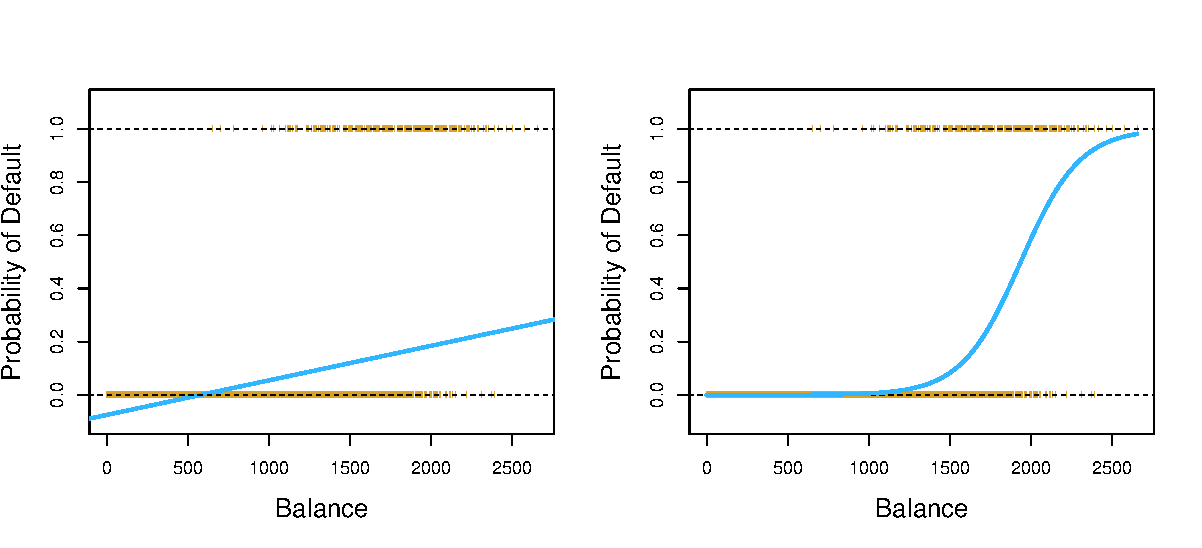
\includegraphics[width=.85\textwidth]{4-2}}

\end{frame}

\begin{frame}{\normalsize Linear/Quadratic Discriminant Analysis}

\begin{itemize}
	\item Linear Discriminant Analysis (LDA)
	\begin{itemize}
	\item Observations from the $k$th class: $X \sim N(\mu_k, \bm{\Sigma})$
	 \includegraphics[width=.8\textwidth]{discrim-lda}
	\end{itemize}

	\item Quadratic Discriminant Analysis (QDA)
	\begin{itemize}
	\item Observations from the $k$th class: $X \sim N(\mu_k, \bm{\Sigma_k})$
	\includegraphics[width=.85\textwidth]{discrim-qda}
	\end{itemize}
\end{itemize}

\end{frame}

\begin{frame}{\normalsize Linear/Quadratic Discriminant Analysis}


\centerline{\includegraphics[width=\textwidth]{4-9}}


\end{frame}

\begin{frame}{Logistic regression and LDA}

\begin{itemize}
	
	\item Logistic regression
	\begin{itemize}
	\item $log(\frac{p(x)}{1 - p(x)}) = \beta_0 + \beta_1 x$
	\item $\beta_0$ and $\beta_1$ estimated using maximum likelihood
	\end{itemize}
	
	\item Linear Discriminant Analysis
	\begin{itemize}
	\item $log(\frac{p_1(x)}{1 - p_1(x)}) = c_0 + c_1 x$
	\item $c_0$ and $c_1$ computed using the estimated mean and variance of a normal distribution
	\end{itemize}
	
	\item[$\rightarrow$] Both logistic regression and LDA produce linear decision boundaries. \textbf{Anything else?} \pause
	\item[$\rightarrow$] However, they make different assumptions and use a different fitting procedure 
	
\end{itemize}
\end{frame}


\begin{frame}{kNN Classifier}

One of the simplest classifiers. Given a test observation $x_0$:
\begin{itemize}
\item Find the $K$ nearest points to $x_0$ in the training data: ${\cal N}_0$.
\item Estimate conditional probabilities
$\text{Pr}(Y=j \mid X=x_0) = \frac{1}{K}\sum_{i\in {\cal N}_0} I(y_i = j).$
\item Classify $x_0$ to class with largest probability.
\item[$\rightarrow$] Nonparametric approach: no assumptions about the shape of the decision boundary
\item[$\rightarrow$] No table of coefficients as in logistic regression
\end{itemize}
\end{frame}

\begin{frame}{kNN Classifier}
\fullwidth{2-14}
\begin{textblock}{10}(0.5,8.4)
$K=3$.
\end{textblock}
\end{frame}

\begin{frame}{kNN Classifier}
\fullwidth{2-16}
\end{frame}


\begin{frame}{kNN Classifier}
\fullheight{2-17}
\end{frame}



\begin{frame}{Maximal Margin Classifier}

   \begin{minipage}[c]{.65\linewidth}
      \includegraphics[width=\textwidth]{9-2}
   \end{minipage} \hfill
   \begin{minipage}[c]{.32\linewidth}
      \includegraphics[width=\textwidth]{9-3}
   \end{minipage}
   
   \begin{minipage}[c]{.68\linewidth}
      \includegraphics[width=\textwidth]{9-5}
   \end{minipage} \hfill
   \begin{minipage}[c]{.28\linewidth}
      \includegraphics[width=\textwidth]{9-4}
   \end{minipage} 
   
%\only<1-2>{ \centerline{\includegraphics[width=.6\textwidth]{9-2} \includegraphics[width=.27\textwidth]{9-3}} }

%\only<2>{ \centerline{\includegraphics[width=.6\textwidth]{9-5}} }

\end{frame}

\begin{frame}{Support Vector Classifier}

{\small We allow ``few'' players from the other team to be on our side (but inside the margin)}

\centerline{\includegraphics[width=.55\textwidth]{9-7}}

\end{frame}

\begin{frame}{Support Vector Classifier}

\centerline{\includegraphics[width=.9\textwidth]{support-vector-classifier}}

\begin{itemize}\small
	\item $M:$ the width of the margin
	\item $C:$ a nonegative tuning parameter
	\item $\epsilon_i$: \emph{slack variables} that allow individual observations to be on the wrong side of the margin or the hyperplane ($\epsilon_i = 0, 0 <\epsilon_i < 1, \epsilon_i > 1$).
\end{itemize}


\end{frame}


\begin{frame}{Support Vector Machines}

\only<1-2>{ \centerline{\includegraphics[width=.7\textwidth]{9-8}} }

\only<2>{  \centerline{\includegraphics[width=.7\textwidth]{9-9}}   }


\end{frame}


\begin{frame}{SVM and logistic regression}

%\centerline{\includegraphics[width=\textwidth]{loss-svm}}
\vspace{-0.5cm}
\centerline{\includegraphics[width=.7\textwidth]{9-12}}


\end{frame}

\begin{frame}{Classification methods}

%\url{https://en.wikipedia.org/wiki/Linear_classifier#Generative_models_vs._discriminative_models}

\begin{itemize}
	\item Logistic regression

	\item Linear Discriminant Analysis
	
	\item Quadratic Discriminant Analysis

	\item k-Nearest Neighbours

	\item Support Vector Machines

	\item Advanced methods: Trees, Boosting and Random Forests (\textcolor{blue}{Week 10})
	\item[$\rightarrow$] \alert{Generative} and \alert{discriminative}  models
\end{itemize}



\end{frame}



\begin{frame}{Which classification method?}

\begin{itemize}
	\item Is it binary or multi-class classification?
	\item How many training examples do we have?
	\item What is the dimensionality of the problem?
	\item How many categorical variables do we have?
	\item Are features independent?
	\item Do we expect the classes to be linearly separable?
	\item Any requirements in terms of computational time/performance/memory usage?
	\item Importance of interpretability?
\end{itemize}

\end{frame}


\begin{frame}{\large Empirical comparison of classifiers}

\begin{itemize}
	\item We compare the following classifiers: \alert{KNN-1}, \alert{KNN-CV}, \alert{LDA}, \alert{Logistic} and \alert{LDA}
	\item We consider \textbf{six different scenarios} for the data generating process
	\item Scenarios 1-3 are \textbf{linear}, and scenarios 4-6 are \textbf{nonlinear}
	\item In each scenario, we generate \textbf{$100$ random training data sets}. For each of these training sets, we fit each model to the data and compute the test error rate on a \textbf{large test set}
\end{itemize}


\end{frame}

\begin{frame}{Scenario 1}

{\small There were 20 training observations in each of two classes. The observations within each class were uncorrelated random normal variables with a different mean in each class.}

\only<2>{\centerline{\includegraphics[width=.42\textwidth]{4-10-1}}}
	
\end{frame}

\begin{frame}{Scenario 2}

Details are as in Scenario 1, except that within each class, the two predictors had a correlation of -0.5.


\only<2>{\centerline{\includegraphics[width=.45\textwidth]{4-10-2}}}
	
\end{frame}

\begin{frame}{Scenario 3}

We generated $X_1$ and $X_2$ from the $t$-distribution, with $50$ observations per class.

\only<2>{\centerline{\includegraphics[width=.45\textwidth]{4-10-3}}}
	
\end{frame}

\begin{frame}{Scenario 4}

The data were generated from a normal distribution, with a correlation of 0.5 between the predictors in the first class, and correlation of -0.5 between the predictors in the second class.

\only<2>{\centerline{\includegraphics[width=.37\textwidth]{4-11-4}}}
	
\end{frame}


\begin{frame}{Scenario 5}

{\small Within each class, the observations were generated from a normal distribution with uncorrelated predictors. However, the responses were sampled from the logistic function using $X_1^2$, $X_2^2$ and $X_1 \times X_2$ as predictors.}

\only<2>{\centerline{\includegraphics[width=.37\textwidth]{4-11-5}}}
	
\end{frame}

\begin{frame}{Scenario 6}

Details are as in the previous scenario, but the responses were sampled from a more complicated non-linear function.

\only<2>{\centerline{\includegraphics[width=.45\textwidth]{4-11-6}}}
	
\end{frame}

\begin{frame}{Summary}\small
	\begin{itemize}
		\item When the true decision boundaries are linear, LDA and logistic regression will perform well
		\item When the boundaries are moderately non-linear, QDA may give better results
		\item For more complicated boundaries, a non-parametric approach such as KNN can be superior
		\item Do not forget the importance of other criteria: number of samples and predictors, computational time, interpretability, etc.
		\item In many data analytics competitions, tree-based methods such as Boosting and Random Forests are often among the best methods (\textcolor{blue}{Week 10})
	\end{itemize}
\end{frame}




\end{document}